\documentclass[aspectratio=169]{../latex_main/tntbeamer}  % you can pass all options of the beamer class, e.g., 'handout' or 'aspectratio=43'
\usepackage{dsfont}
\usepackage{bm}
\usepackage[english]{babel}
\usepackage[T1]{fontenc}
%\usepackage[utf8]{inputenc}
\usepackage{graphicx}
\graphicspath{ {./figures/} }
\usepackage{algorithm}
\usepackage[ruled,vlined,algo2e,linesnumbered]{algorithm2e}
\usepackage{hyperref}
\usepackage{booktabs}
\usepackage{mathtools}

\usepackage{amsmath,amssymb}

\DeclareMathOperator*{\argmax}{arg\,max}
\DeclareMathOperator*{\argmin}{arg\,min}

\usepackage{amsbsy}
\newcommand{\vect}[1]{\bm{#1}}
%\newcommand{\vect}[1]{\boldsymbol{#1}}

\usepackage{pgfplots}
\pgfplotsset{compat=1.16}
\usepackage{tikz}
\usetikzlibrary{trees} 
\usetikzlibrary{shapes.geometric}
\usetikzlibrary{positioning,shapes,shadows,arrows,calc,mindmap}
\usetikzlibrary{positioning,fadings,through}
\usetikzlibrary{decorations.pathreplacing}
\usetikzlibrary{intersections}
\pgfdeclarelayer{background}
\pgfdeclarelayer{foreground}
\pgfsetlayers{background,main,foreground}
\tikzstyle{activity}=[rectangle, draw=black, rounded corners, text centered, text width=8em]
\tikzstyle{data}=[rectangle, draw=black, text centered, text width=8em]
\tikzstyle{myarrow}=[->, thick, draw=black]

% Define the layers to draw the diagram
\pgfdeclarelayer{background}
\pgfdeclarelayer{foreground}
\pgfsetlayers{background,main,foreground}

% Requires XeLaTeX or LuaLaTeX
%\usepackage{unicode-math}

\usepackage{fontspec}
%\setsansfont{Arial}
\setsansfont{RotisSansSerifStd}[ 
Path=../latex_main/fonts/,
Extension = .otf,
UprightFont = *-Regular,  % or *-Light
BoldFont = *-ExtraBold,  % or *-Bold
ItalicFont = *-Italic
]
\setmonofont{Cascadia Mono}[
Scale=0.8
]

% scale factor adapted; mathrm font added (Benjamin Spitschan @TNT, 2021-06-01)
%\setmathfont[Scale=1.05]{Libertinus Math}
%\setmathrm[Scale=1.05]{Libertinus Math}

% other available math fonts are (not exhaustive)
% Latin Modern Math
% XITS Math
% Libertinus Math
% Asana Math
% Fira Math
% TeX Gyre Pagella Math
% TeX Gyre Bonum Math
% TeX Gyre Schola Math
% TeX Gyre Termes Math

% Literature References
\newcommand{\lit}[2]{\href{#2}{\footnotesize\color{black!60}[#1]}}

%%% Beamer Customization
%----------------------------------------------------------------------
% (Don't) Show sections in frame header. Options: 'sections', 'sections light', empty
\setbeamertemplate{headline}{empty}

% Add header logo for normal frames
\setheaderimage{
	% 
\includegraphics[height=\logoheight]{figures/TNT_darkv4.pdf}
	
\includegraphics[height=\logoheight]{../latex_main/figures/luh_logo_rgb_0_80_155.pdf}
	% 
\includegraphics[height=\logoheight]{figures/logo_tntluh.pdf}
}

% Header logo for title page
\settitleheaderimage{
	% 
\includegraphics[height=\logoheight]{figures/TNT_darkv4.pdf}
	
\includegraphics[height=\logoheight]{../latex_main/figures/luh_logo_rgb_0_80_155.pdf}
	% 
\includegraphics[height=\logoheight]{figures/logo_tntluh.pdf}
}

% Title page: tntdefault 
\setbeamertemplate{title page}[tntdefault]  % or luhstyle
% Add optional title image here
%\addtitlepageimagedefault{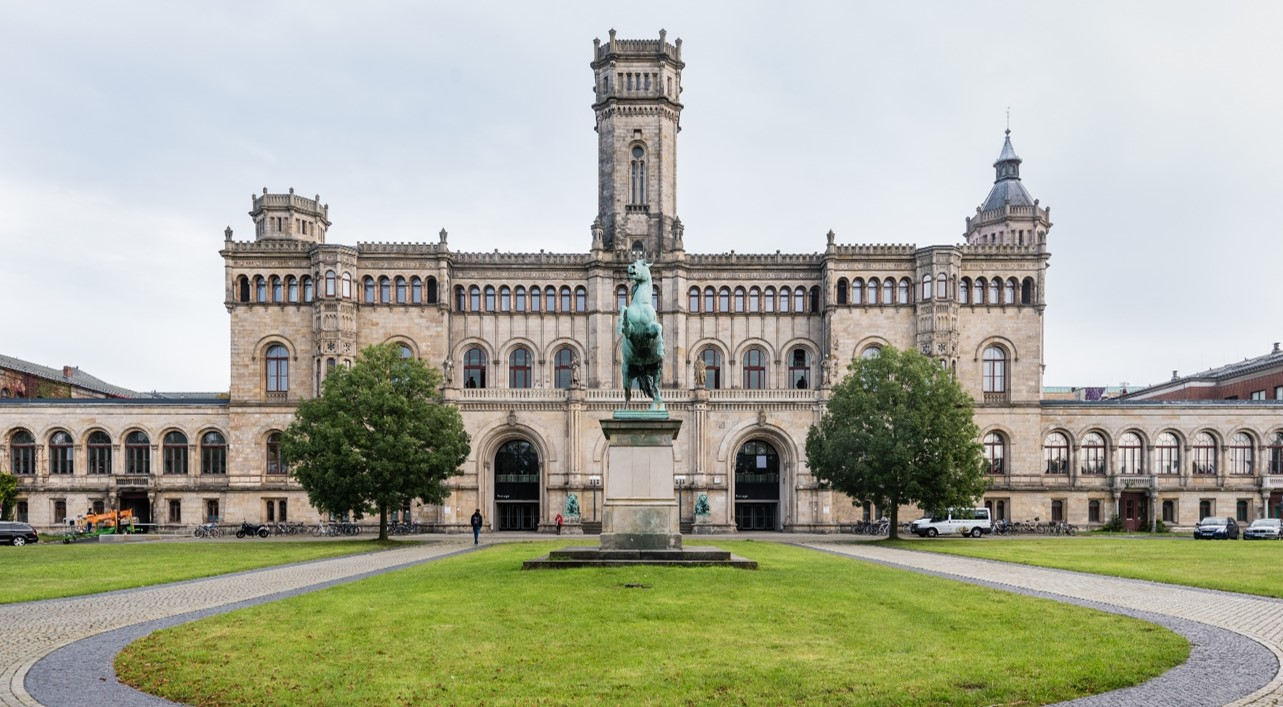
\includegraphics[width=0.65\textwidth]{figures/luh_default_presentation_title_image.jpg}}

% Title page: luhstyle
% \setbeamertemplate{title page}[luhstyle]
% % Add optional title image here
% \addtitlepageimage{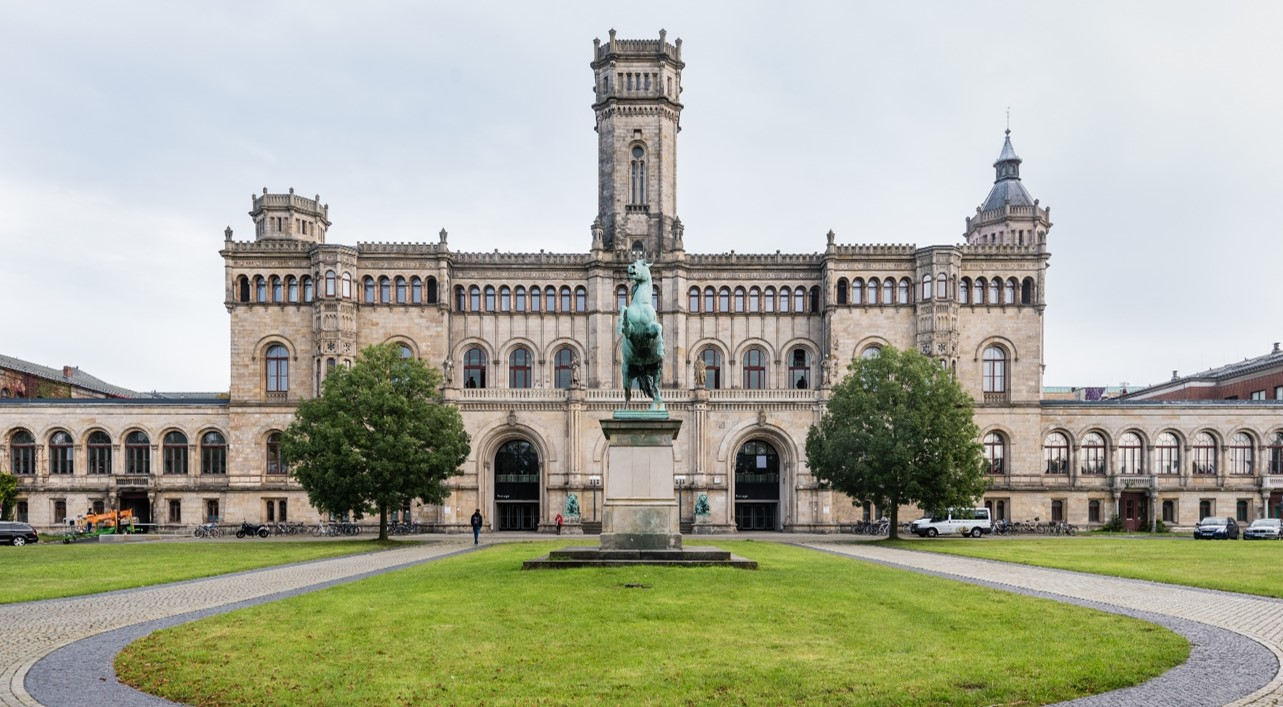
\includegraphics[width=0.75\textwidth]{figures/luh_default_presentation_title_image.jpg}}

\author[Abedjan \& Lindauer]{Ziawasch Abedjan \& Marius Lindauer\\[1em]
	
\includegraphics[height=\logoheight]{../latex_main/figures/luh_logo_rgb_0_80_155.pdf}\qquad
	
\includegraphics[height=\logoheight]{../latex_main/figures/DBIS_Kurzlogo.png}\qquad

\includegraphics[height=\logoheight]{../latex_main/figures/TNT_darkv4}\qquad

\includegraphics[height=\logoheight]{../latex_main/figures/L3S.jpg}	}
\date{Summer Term 2022; \hspace{0.5em} {
\includegraphics[height=1.5em]{../latex_main/figures/Cc-by-nc-sa_icon.svg.png}}; based on \href{https://ds100.org/fa21/}{[DS100]}
}


%%% Custom Packages
%----------------------------------------------------------------------
% Create dummy content
\usepackage{blindtext}

% Adds a frame with the current page layout. Just call \layout inside of a frame.
\usepackage{layout}


%%% Macros
%\renewcommand{\vec}[1]{\mathbf{#1}}
% \usepackage{bm}
%\let\vecb\bm

\title[Semi-Supervised Learning]{DS: Learning}
\subtitle{Semi-Supervised Learning}

\graphicspath{ {./figure/} }
%\institute{}


\begin{document}
	
    \maketitle
    
    \begin{frame}[c]{What is Semi-Supervised Learning?}
        \begin{itemize}
            \item Semi-supervised learning considers learning $f: x \mapsto y$ from training data $\mathcal{D}= \{(x_i,y_i)\}_{i}$ 
            \item \alert{Important:} For some of the $x_i$, the label $y_i$ is unknown.
            \begin{itemize}
                \item Typically, only a small amount of data is labeled and most of the data is unlabeled.
                \item Often the case, if data labeling is very expensive or difficult.
            \end{itemize}
        \end{itemize} 

        \centering
        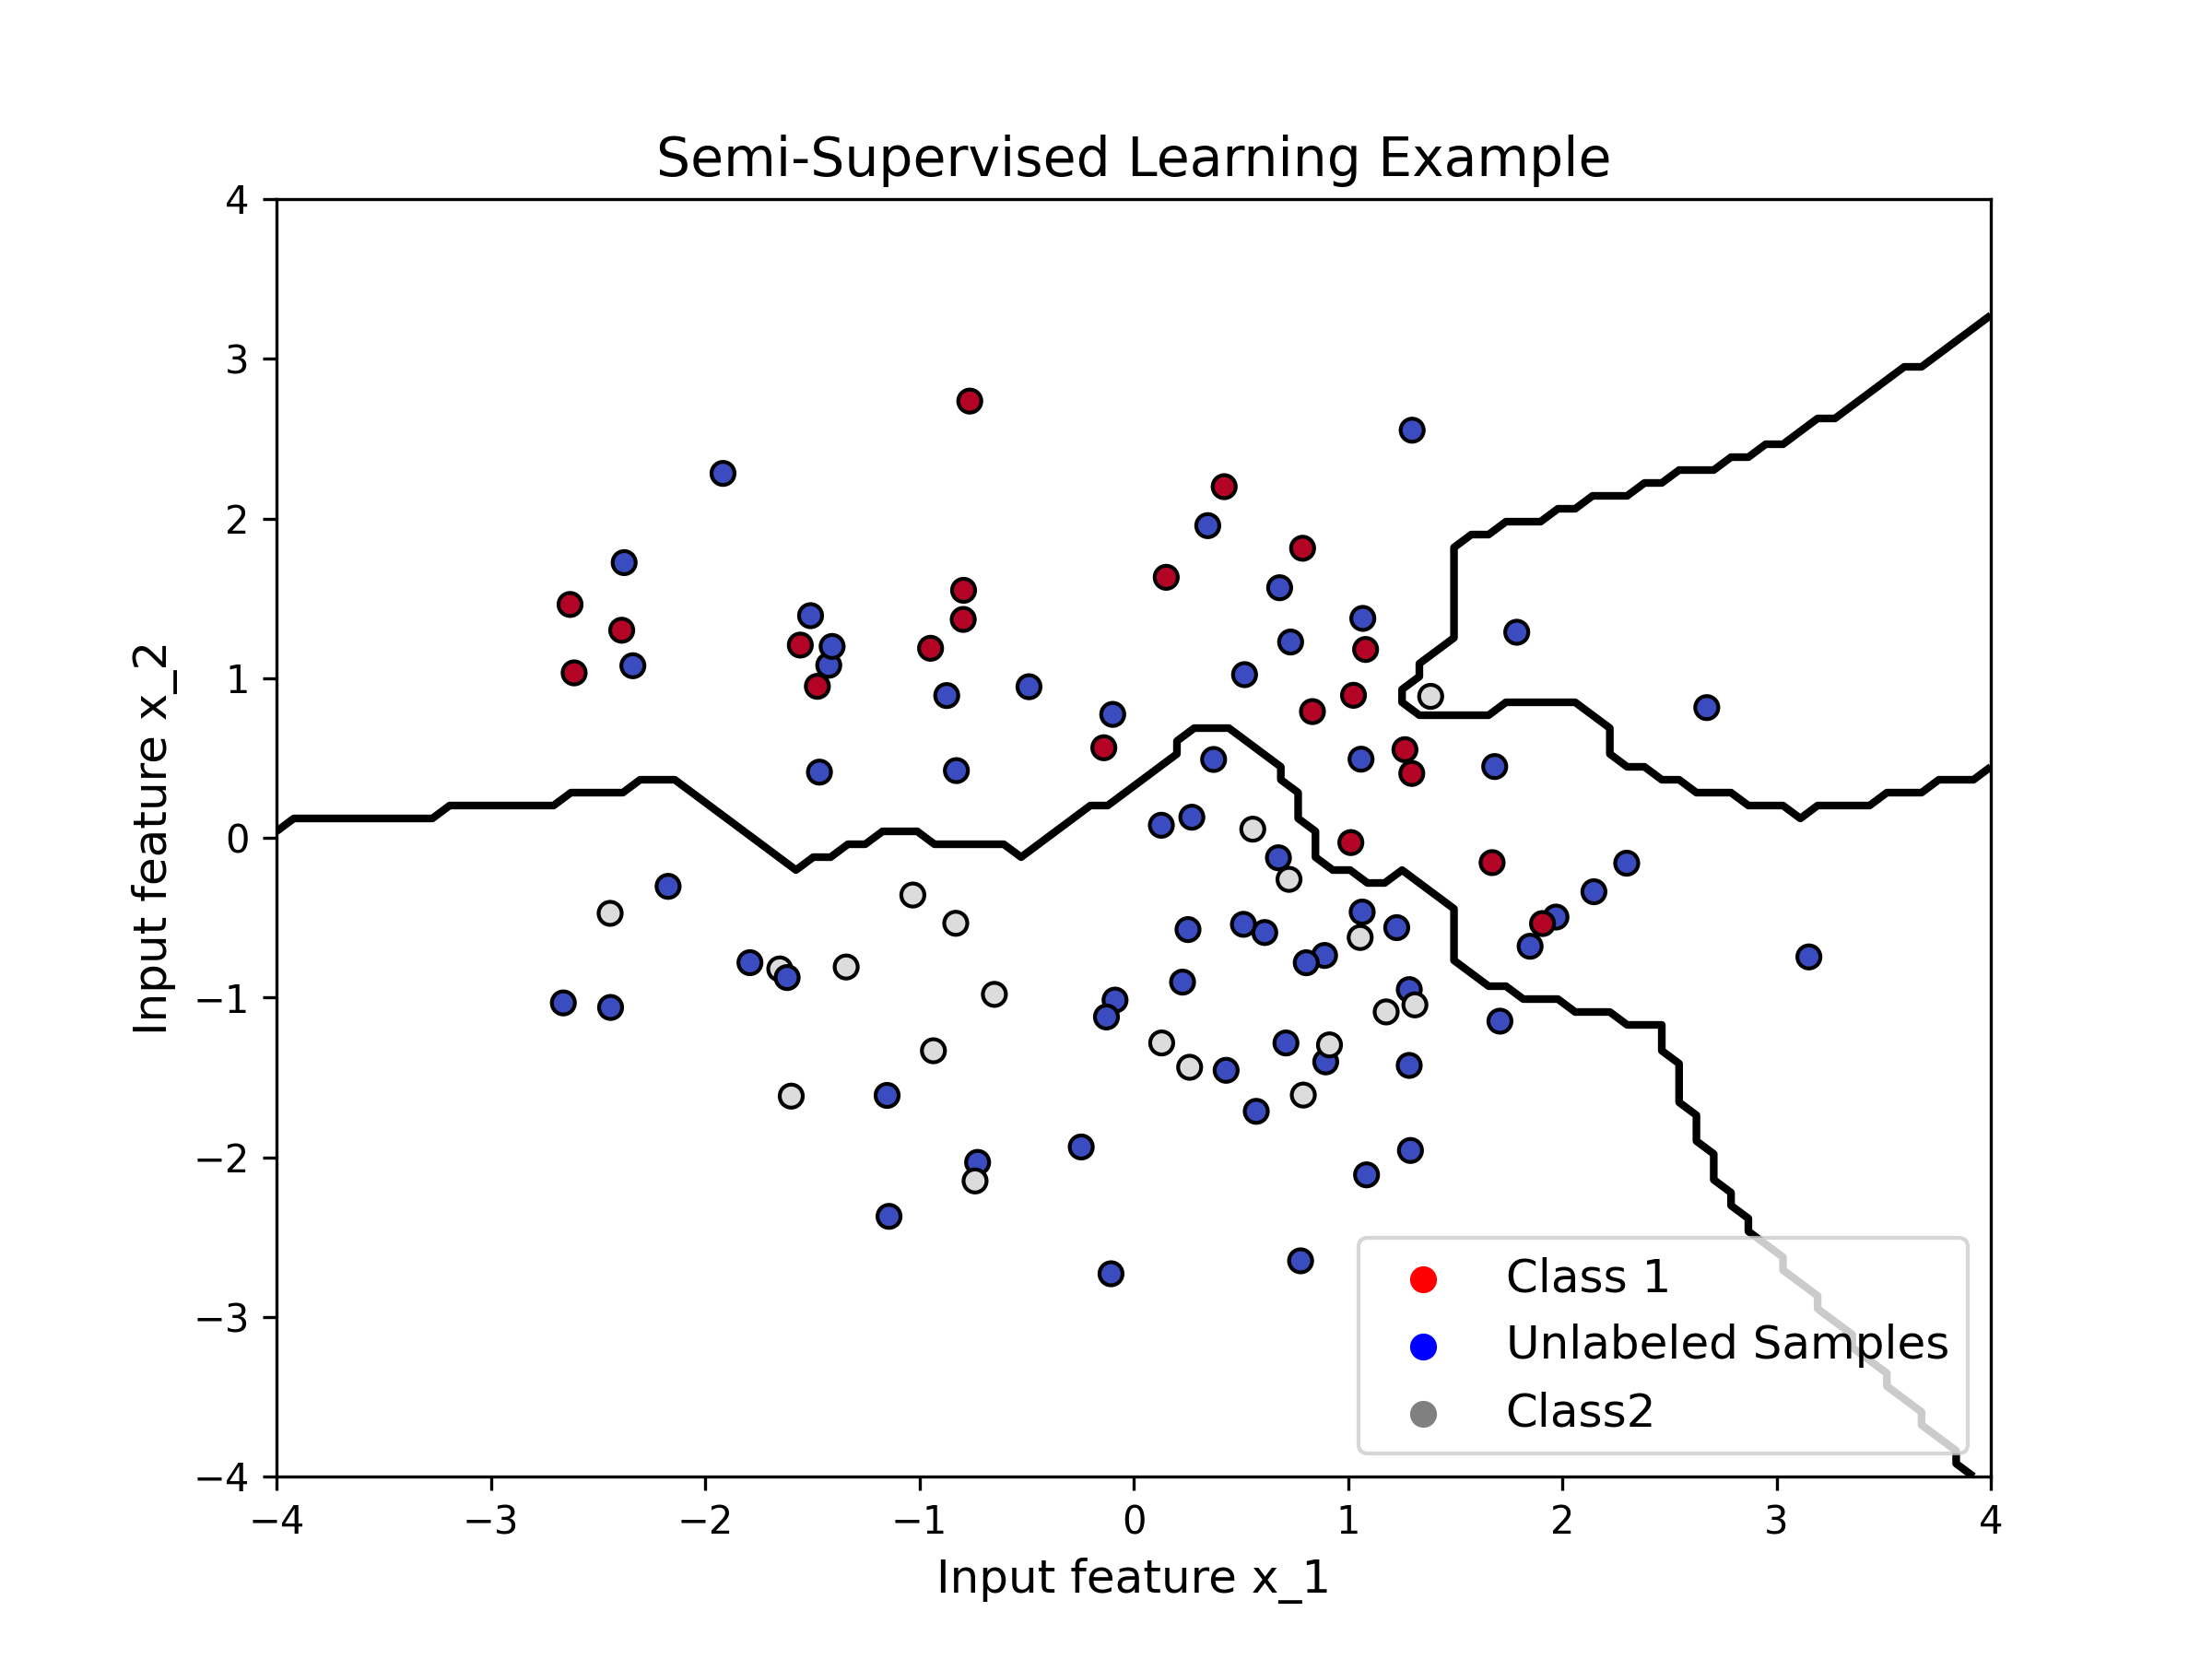
\includegraphics[width=0.46\textwidth]{figure/semi-supervised}

    % import numpy as np
    % import matplotlib.pyplot as plt
    % from sklearn.datasets import make_classification
    % from sklearn.semi_supervised import LabelPropagation
    
    % # generate some random data
    % X, y = make_classification(n_classes=2, n_samples=100, n_features=2, n_redundant=0, n_informative=2, n_clusters_per_class=1)
    
    % # set labels for only a few samples
    % y[20:80] = -1
    
    % # fit a semi-supervised learning model
    % model = LabelPropagation()
    % model.fit(X, y)
    
    % # create a grid of points to evaluate the model
    % xx, yy = np.meshgrid(np.linspace(-4, 4, 100), np.linspace(-4, 4, 100))
    % Z = model.predict(np.c_[xx.ravel(), yy.ravel()])
    % Z = Z.reshape(xx.shape)
    
    % # plot the data and the decision boundary
    % plt.figure(figsize=(8,6), dpi=100)
    % plt.scatter(X[:,0], X[:,1], c=y, cmap='coolwarm', edgecolors='k')
    % plt.contour(xx, yy, Z, levels=[0], linewidths=2, colors='black')
    % plt.xlabel('Input feature x_1', fontsize=12)
    % plt.ylabel('Input feature x_2', fontsize=12)
    % plt.title('Semi-Supervised Learning Example', fontsize=14)
    % plt.legend(handles=[plt.scatter([],[],color='red', label='Class 1'),
    %                      plt.scatter([],[],color='blue', label='Unlabeled Samples'),
    %                      plt.scatter([],[],color='gray', label='Class2')],
    %            loc='lower right', fontsize=12)
    % plt.show()


    \end{frame}

    \begin{frame}{Exemplary Semi-Supervised Learning: Label Propagation}

        \begin{itemize}
            \item  Propagate the labels from labeled data points to unlabeled data points based on their similarity in feature space.
            \item assumes that similar data points should have similar labels.
            \item Constructs a graph, where each data point is a node and edges are added between neighboring data points. The weight of each edge is determined by the similarity between the two data points.
            \item Iteratively assigns labels to the unlabeled data points based on the labels of the labeled data points that are most similar to them in feature space.
            \item Often used for scenarios where labeled data is scarce but large amounts of unlabeled data are available.
        \end{itemize}
        
    \end{frame}

    
    \begin{frame}[c]{Semi-Supervised Learning with Two Loss Functions}

    \begin{description}
        \item[Supervised loss] is calculated on the labeled data points and it measures the difference between the predicted output and the true output. Eg. mean squared error (MSE), cross-entropy loss, and hinge loss.
        \item[Unsupervised loss] is calculated on the entire dataset, including both labeled and unlabeled data points. It encourages the model to learn a smooth representation of the input space, so that similar inputs are mapped to similar feature representations. E.g. reconstruction loss, mutual information loss, and contrastive loss.]
    \end{description}

    \pause
    \medskip

    $\leadsto$ By combining both supervised and unsupervised loss functions, semi-supervised learning approaches can leverage both labeled and unlabeled data points to improve the model's performance.
    
    \end{frame}






\end{document}